% !TeX root = 机械设计.tex
% ============================================================
%  第一章 机械设计概论
%  来源：教材/机械设计《机械原理与机械设计（下）》读书笔记
%  说明：正文表述与公式均沿用原文，仅作版式与环境归类
% ============================================================
\chapter{机械设计概论}
\label{chap:机械设计概论}

\section{机器、机械与机械零件}
\label{sec:机器机械与机械零件}

\begin{definition}[机器]
\label{def:机器}
\textbf{机器}(\emph{machine})是人类进行生产以减轻体力劳动和提高劳动生产率的主要工具。
\end{definition}

\begin{definition}[机械]
\label{def:机械}
\textbf{机械}(\emph{machinery})是机器和机构(\emph{mechanism})的总称。使用机械进行生产的水平是衡量一个国家的技术水平和现代化程度的重要标志之一。
\end{definition}

\begin{definition}[零件与部件]
\label{def:零件与部件}
组成机器的不可拆的基本单元称为\textbf{机械零件}(\emph{machine elements})或简称\textbf{零件}；为完成特定的功能在结构上组合在一起并协同工作的零件组合称为\textbf{部件}(\emph{mechanical components})，如联轴器、轴承、减速器等。机械零件一般泛指零件与部件。
\end{definition}

\begin{figure}[H]
\centering
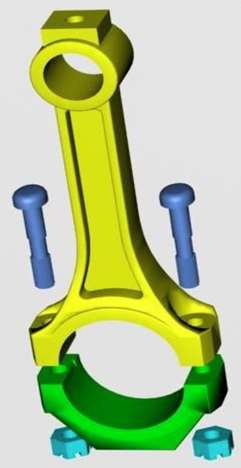
\includegraphics[width=0.5\textwidth]{Figure/零件示意图.png}
\caption{零件示意图（连杆组件装配示意）}
\label{fig:零件示意图}
\end{figure}

\begin{figure}[H]
\centering
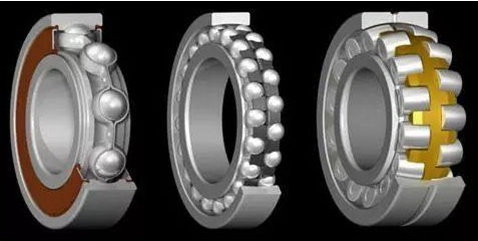
\includegraphics[width=0.85\textwidth]{Figure/轴承部件图.png}
\caption{轴承部件图（几种滚动轴承剖面模型）}
\label{fig:轴承部件图}
\end{figure}

\begin{definition}[通用零件与专用零件]
\label{def:通用零件与专用零件}
各种机器中普遍使用的零件称\textbf{通用零件}(\emph{universal components})，如螺钉、键、带、齿轮、轴、弹簧等；只在特定的机器上使用的零件称为\textbf{专用零件}(\emph{special components})，如发动机的曲轴、汽轮机的叶片、船用螺旋桨等都是专用零件。
\end{definition}

\begin{definition}[机构]
\label{def:机构}
\textbf{机构}(\emph{mechanism})是能实现预期的机械运动的实物组合。机械的共同特征为：（1）人为的实物组合；（2）其组成各部分之间具有确定的相对运动；（3）必须能做有用功，完成信息的传递及能量的转换。机构仅具有特征（1）（2），机器能做有用功，而机构不能，仅能实现预期的机械运动；机器是由一个或多个机构组成的系统。
\end{definition}

\begin{definition}[机器]
\label{def:机器组成}
\textbf{机器}通常由以下部分组成：
\begin{enumerate}
	\item 原动机：机械动力的来源；
	\item 执行机构：完成机械预期的动作；
	\item 传动机构：把原动机的运动和功率传递给工作机的中间环节；
	\item 自动控制部分（控制系统）。
\end{enumerate}
\end{definition}

\begin{definition}[构件]
\label{def:构件}
\textbf{构件}是组成机器的运动单元体，具有确定的运动。按照其在机器中所起的作用可分为：
\begin{enumerate}
	\item 机架：固定不动的构件；
	\item 原动件（输入构件）：驱动力（矩）作用的构件；
	\item 从动件（输出构件）：随着原动构件的运动而运动的构件。
\end{enumerate}
\end{definition}

\section{标准化、系列化与通用化}
\label{sec:三化}

\begin{definition}[标准化]
\label{def:标准化}
在不同类型、不同规格的各种机器中，将同类零件或部件的结构型式、尺寸、材料等限定在合理的数量范围内，称为\textbf{标准化}(\emph{standardization})。
\end{definition}

\begin{definition}[标准件与非标准件]
\label{def:标准件}
按规定标准生产并给以标准代号的零件和部件称为\textbf{标准件}(\emph{standard components})，不按规定标准生产的零件和部件称为\textbf{非标准件}。
\end{definition}

\begin{definition}[系列化]
\label{def:系列化}
根据要求，按一定规律优化组合零、部件系列，称为\textbf{系列化}。系列化是标准化的重要内容，如螺栓系列、滚动轴承的类型和尺寸系列等。
\end{definition}

\begin{definition}[通用化]
\label{def:通用化}
最大限度地减少和合并零、部件的型式、尺寸和材料品种等，称为\textbf{通用化}(\emph{universalization})。
\end{definition}

\begin{keybox}[三化]
标准化、系列化、通用化通称\textbf{三化}。
\end{keybox}

\section{机械设计的基本要求}
\label{sec:机械设计的基本要求}

\subsection{对机器设计的基本要求}

\textbf{（1）对机器使用功能方面的要求。}

\begin{enumerate}
	\item 实现预定的使用功能是机器设计的最基本的要求，
	\item 好的使用性能指标是设计的主要目标。
	\item 操作使用方便、工作安全可靠、体积小、重量轻、效率高、外形美观、噪声低等往往也是机器设计时所要求的。
	\item 对不同用途的机器还可能提出一些特殊的要求，如巨型机器有起重运输的要求，对生产食品的机器有保持清洁和不污染环境的要求等。
\end{enumerate}

\textbf{（2）对机器经济性的要求。}

\begin{enumerate}
	\item 设计的经济性体现为合理的功能定位、实现使用功能要求的最简单的技术途径和最简单、合理的结构；
	\item 制造的经济性体现为采用合理的加工制造工艺、尽可能采用新的制造技术和最佳的生产组织管理，从而使机器在保证设计功能的前提下有尽可能低的制造成本；
	\item 使用的经济性表现为机器应有较高的生产率、高效率，较少地消耗能源、原材料和辅助材料，管理和维护保养方便、费用低。
\end{enumerate}

\subsection{对机械零件设计的基本要求}

\begin{enumerate}
	\item 要求在预定的工作期限内正常可靠地工作，从而保证机器的各种功能的正常实现；
	\item 要尽量降低零件的生产制造成本。
\end{enumerate}

\section{机械设计的一般程序}
\label{sec:机械设计的一般程序}

\subsection{机器设计的一般程序}

机器设计一般划分为市场调研与可行性研究、原理方案设计、技术设计、改进设计四个阶段，各阶段均设有评价与反馈环节，其流程如图~\ref{fig:机器设计一般程序} 所示。

\begin{figure}[H]
\centering
\begin{tikzpicture}[
	stage/.style={draw=structurecolor!65, fill=structurecolor!5, rounded corners=3pt,
		text width=2.4cm, align=center, font=\scriptsize, inner sep=3pt, minimum height=1.1cm},
	goal/.style={draw=gold!82!black, fill=gold!12, rounded corners=3pt,
		text width=2.4cm, align=center, font=\scriptsize, inner sep=3pt, minimum height=1.1cm},
	judge/.style={diamond, aspect=2.1, draw=structurecolor!65, fill=structurecolor!5,
		text width=1.6cm, align=center, font=\scriptsize, inner sep=1pt},
	lab/.style={font=\small\heiti, text=structurecolor, anchor=west},
	arrow/.style={-{Stealth[length=2.1mm]}, line width=0.7pt, draw=structurecolor!80},
	back/.style={-{Stealth[length=2.1mm]}, line width=0.7pt, draw=warnColor, dashed}
]
	% ---------- 第一阶段 ----------
	\node[lab] at (0,1.35) {第一阶段：市场调研、可行性研究};
	\node[stage] (a1) at (1.4,0)    {社会需求调研};
	\node[stage] (a2) at (4.4,0)    {提出设计任务};
	\node[stage] (a3) at (7.4,0)    {可行性研究};
	\node[stage] (a4) at (10.4,0)   {明确设计任务};
	\node[goal]   (a5) at (13.4,0)   {设计任务书};
	\draw[arrow] (a1) -- (a2);
	\draw[arrow] (a2) -- (a3);
	\draw[arrow] (a3) -- (a4);
	\draw[arrow] (a4) -- (a5);

	% ---------- 第二阶段 ----------
	\node[lab] at (0,-1.85) {第二阶段：原理方案设计（\emph{schematic design}）};
	\node[stage]  (b1) at (1.4,-3.2)  {机器的功能定位};
	\node[stage]  (b2) at (4.4,-3.2)  {可行的技术\\途径分析};
	\node[judge]  (b3) at (7.4,-3.2)  {方案综合评价};
	\node[goal]    (b4) at (10.4,-3.2) {确定最佳原理方案};
	\draw[arrow] (a1) -- (b1);
	\draw[arrow] (b1) -- (b2);
	\draw[arrow] (b2) -- (b3);
	\draw[arrow] (b3) -- node[above, font=\tiny]{Y} (b4);
	\draw[back]  (b3.north) -- (7.4,-2.2) -- (0,-2.2) -- (0,-3.2)
		node[midway, above, font=\tiny]{N} -- (b1.west);

	% ---------- 第三阶段 ----------
	\node[lab] at (0,-5.05) {第三阶段：技术设计（\emph{technical design}）};
	\node[stage] (c1) at (1.4,-6.4)  {造型、结构\\方案设计};
	\node[judge] (c2) at (4.4,-6.4)  {结构方案评价};
	\node[stage] (c3) at (7.4,-6.4)  {最佳结构方案};
	\node[stage] (c4) at (10.4,-6.4) {总体设计};
	\node[stage] (c5) at (10.4,-8.6) {零部件设计};
	\node[stage] (c6) at (7.4,-8.6)  {编制技术文件};
	\node[goal]   (c7) at (4.4,-8.6)  {总装图、部件图、零件工作图、设计计算书、零件明细表和其他技术文件};
	\draw[arrow] (b1) -- (c1);
	\draw[arrow] (c1) -- (c2);
	\draw[arrow] (c2) -- node[above, font=\tiny]{Y} (c3);
	\draw[arrow] (c3) -- (c4);
	\draw[arrow] (c4) -- (c5);
	\draw[arrow] (c5) -- (c6);
	\draw[arrow] (c6) -- (c7);
	\draw[back]  (c2.south) -- (4.4,-7.5) -- (0,-7.5) -- (0,-6.4)
		node[midway, above, font=\tiny]{N} -- (c1.west);

	% ---------- 第四阶段 ----------
	\node[lab] at (0,-10.05) {第四阶段：改进设计（样机试制、试验）};
	\node[stage] (d1) at (1.4,-11.6)  {样机试制与试验};
	\node[judge] (d2) at (4.4,-11.6)  {样机综合评价};
	\node[stage] (d3) at (7.4,-11.6)  {信息反馈\\修改设计};
	\node[goal]   (d4) at (10.4,-11.6) {考核设计功能，完善设计方案};
	\draw[arrow] (c7.south) -- (4.4,-9.9) -- (1.4,-9.9) -- (d1.north);
	\draw[arrow] (d1) -- (d2);
	\draw[arrow] (d2) -- node[above, font=\tiny]{N} (d3);
	\draw[arrow] (d2.east) -- (7.4,-10.5) -- (10.4,-10.5)
		node[midway, above, font=\tiny]{Y} -- (d4.north);
	\draw[back]  (d3.north) -- (7.4,-10.3) -- (0,-10.3) -- (0,-11.6) -- (d1.west);
\end{tikzpicture}
\caption{机器设计的一般程序}
\label{fig:机器设计一般程序}
\end{figure}

\subsection{机械零件设计的一般步骤}

\begin{enumerate}
	\item 根据机器的工作情况，按力学方法建立零件简化的力学模型，确定零件上的计算载荷。

	根据原动机的额定功率或根据机器在稳定和理想工作条件下的工作阻力，按力学方法计算出的作用在零件上的载荷称为\textbf{名义载荷}（或称公称载荷、额定载荷）。考虑原动机与工作机间实际载荷随时间的变化、载荷在零件上分布的不均匀性及其他影响零件受力等因素的影响，引入载荷系数 $K$（或工作情况系数）来作概略估计。载荷系数 $K$ 与名义载荷的乘积称为\textbf{计算载荷}。

	\item 根据零件的使用要求，选择零件的类型与结构。

	\item 根据零件的工作条件和材料的力学性能等选择适当的零件材料。

	\item 据零件可能的失效形式确定计算准则，并根据零件的工作能力准则，确定零件的基本尺寸，并加以标准化和圆整。

	\item 根据工艺性和标准化等原则进行零件的结构设计。

	\item 绘制零件工作图，并编写计算说明书。
\end{enumerate}

\begin{definition}[名义载荷与计算载荷]
\label{def:名义载荷与计算载荷}
根据原动机的额定功率或根据机器在稳定和理想工作条件下的工作阻力，按力学方法计算出的作用在零件上的载荷称为\textbf{名义载荷}（或称公称载荷、额定载荷）；载荷系数 $K$（或工作情况系数）与名义载荷的乘积称为\textbf{计算载荷}。
\end{definition}

\subsection{设计计算与校核计算}

\begin{sloppypar}
机械零件的计算可分为\textbf{设计计算}（\emph{design calculation}）和\textbf{校核计算}（\emph{checking calculation}）两种。
\end{sloppypar}

\begin{definition}[设计计算]
\label{def:设计计算}
先根据零件的工作情况和选定的工作能力准则拟定出安全条件，用计算方法求出零件危险截面的尺寸，然后根据结构和工艺要求，确定具体的零件结构。
\end{definition}

\begin{definition}[校核计算]
\label{def:校核计算}
先参照已有的零件实物、图纸或根据经验初步拟定零件的结构和基本尺寸，然后根据工作能力准则校核危险截面是否安全。
\end{definition}

\begin{note}
校核计算时，因为已知零件的有关尺寸和结构，所以计算结果一般较精确。
\end{note}

\section{机械零件的主要失效形式和设计计算准则}
\label{sec:失效形式与设计计算准则}

\subsection{机械零件的失效形式}

\begin{definition}[失效]
\label{def:失效}
\textbf{失效}(\emph{failure})：机械零件丧失正常工作能力或达不到设计要求的性能时称为失效。
\end{definition}

机械失效形式虽然有很多种，但归结起来可以总结为以下问题：

\begin{enumerate}
	\item 强度
	\item 刚度
	\item 耐磨性
	\item 温度对工作能力的影响
	\item 振动稳定性
	\item 可靠性
\end{enumerate}

\begin{figure}[H]
\centering
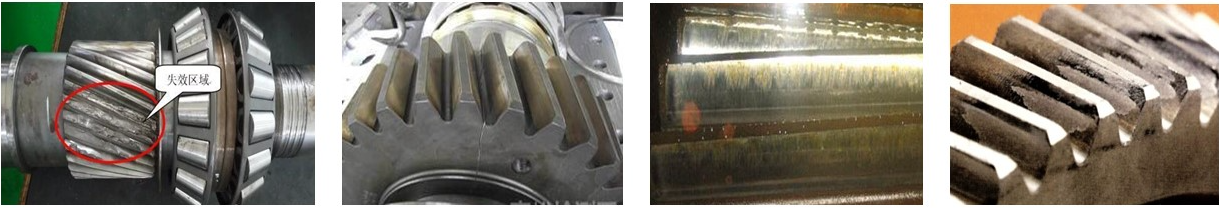
\includegraphics[width=\textwidth]{Figure/一些失效案例.png}
\caption{齿轮类零件的失效案例}
\label{fig:失效案例}
\end{figure}

\subsection{机械零件的计算准则}

\begin{definition}[工作能力]
\label{def:工作能力}
零件不发生失效时的安全工作限度称为\textbf{工作能力}。
\end{definition}

\begin{definition}[计算准则]
\label{def:计算准则}
\textbf{计算准则}（\emph{criterion}）：根据零件失效分析结果，以防止产生各种可能失效为目的，拟定的零件工作能力计算依据的基本原则。
\end{definition}

\textbf{1. 强度准则}

\begin{definition}[强度]
\label{def:强度}
\textbf{强度}(\emph{strength})是指零件抵抗破坏的能力。强度准则要求零件中的应力不超过许用极限，其表达式为
\begin{equation}
	\sigma \leq [\sigma]=\frac{\sigma_{\lim }}{S_{\sigma}}
	\label{eq:概论:正应力强度准则}
\end{equation}
\begin{equation}
	\tau \leq [\tau]=\frac{\tau_{\lim }}{S_{\tau}}
	\label{eq:概论:切应力强度准则}
\end{equation}
\end{definition}

\textbf{2. 刚度准则}

\begin{definition}[刚度]
\label{def:刚度}
\textbf{刚度}(\emph{rigidity})是零件在载荷作用下抵抗弹性变形的能力。刚度准则要求为：零件的弹性变形 $y$ 小于或等于许用的弹性变形量 $[y]$。其表达式为
\begin{equation}
	y \leq [y]
	\label{eq:概论:刚度准则}
\end{equation}
\end{definition}

\textbf{3. 耐磨性准则}

\begin{definition}[耐磨性]
\label{def:耐磨性}
\textbf{耐磨性}(\emph{wear resistance})是作相对运动的零件及其工作表面抵抗磨损的能力。耐磨性准则要求零件工作表面的压强及压强—速度乘积不超过许用值，即
\begin{equation}
	p \leq [p]
	\label{eq:概论:压强准则}
\end{equation}
\begin{equation}
	pv \leq [pv]
	\label{eq:概论:pv准则}
\end{equation}
其中，$p$ 为工作压强，$[p]$ 为许用压强；$pv$ 为压强—速度乘积，$[pv]$ 为许用 $pv$ 值。
\end{definition}

\begin{note}
正常磨损是指磨损速度稳定缓慢，在预定的使用期限内，零件的磨损量不超过允许值。
\end{note}

\textbf{4. 振动与噪声准则}

\begin{definition}[振动与噪声准则]
\label{def:振动与噪声准则}
对高速机械或对噪声有严格要求的机械，应进行振动分析和计算，确定机械或零件的固有频率 $f$ 或强迫振动频率 $f_p$，并分析噪声源。为保证机械能稳定工作，应避免共振，即
\begin{equation}
	\begin{cases}
		f_p < 0.85f \\[0.5em]
		f_p > 1.15f
	\end{cases}
	\label{eq:概论:振动准则}
\end{equation}
其中，$f$ 为固有频率，$f_p$ 为强迫振动频率。
\end{definition}

\begin{note}
不满足上述条件时，可改变机械或零件的刚度，或采取减振措施。
\end{note}

\textbf{5. 热平衡准则}

\begin{definition}[热平衡准则]
\label{def:热平衡准则}
工作时发生剧烈摩擦的零件，其摩擦部位会产生大量的热。若散热不良，则零件的温度升高，会破坏正常的润滑条件、使零件承载能力降低，并引起热变形及热应力。热平衡准则要求：达到热平衡时，机械或零件的温升不超过正常工作允许的最大温升。
\end{definition}

\textbf{6. 可靠性准则}

\begin{definition}[可靠度]
\label{def:可靠度}
在规定的工作条件下和预定的工作期限内，零件正常工作（不发生失效）的概率称为\textbf{可靠度}，即
\begin{equation}
	R_t = \frac{N_t}{N} = \frac{N-N_f}{N} = 1-\frac{N_f}{N}
	\label{eq:概论:可靠度}
\end{equation}
\end{definition}

\begin{definition}[不可靠度]
\label{def:不可靠度}
零件失效的概率称为\textbf{不可靠度}（失效概率），即
\begin{equation}
	F_t = \frac{N_f}{N} = 1 - R_t
	\label{eq:概论:不可靠度}
\end{equation}
其中，$N$ 为零件总数量，$N_t$ 为正常工作零件数，$N_f$ 为失效零件数。
\end{definition}

\begin{note}
由多个零件组成的串联系统，任一零件失效都会引起整个系统的失效，整个机器的可靠度为
\begin{equation}
	R = R_1 R_2 \cdots R_n
	\label{eq:概论:串联系统可靠度}
\end{equation}
机械零件可靠性水平的高低，直接影响机械系统的可靠性。
\end{note}

\section{机械零件的常用材料}
\label{sec:常用材料}

\subsection{常用材料}

\subsubsection{黑色金属（铁基）}

\begin{enumerate}
	\item \textbf{灰铸铁}：铸造性好、减震耐磨、成本低，多用于机座、箱体、床身；
	\item \textbf{球墨铸铁}：强度韧性优于普通铸铁，可替代部分钢材，用于制造曲轴、齿轮；
	\item \textbf{可锻铸铁}：塑性韧性较好，适合薄壁复杂小件；
	\item \textbf{铸钢}：强度高，适合承受大载荷的铸造零件；
	\item \textbf{碳钢、合金钢}：机械中使用最多，可热处理强化，用于轴、齿轮、螺栓等受力零件。
\end{enumerate}

\begin{figure}[H]
\centering
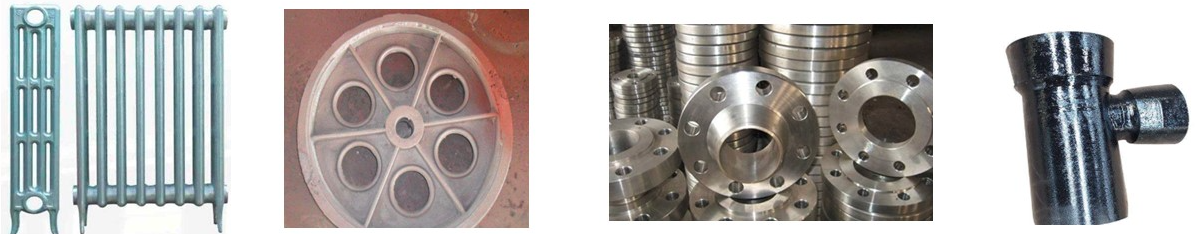
\includegraphics[width=0.95\textwidth]{Figure/黑色金属材料.png}
\caption{黑色金属材料示例}
\label{fig:黑色金属材料}
\end{figure}

\subsubsection{有色金属（非铁金属）}

\begin{enumerate}
	\item \textbf{铝合金}：密度小、可减重，用于壳体、支架；
	\item \textbf{铜合金（黄铜、青铜）}：减摩耐磨、导热导电，用于轴承、蜗轮、垫片；
	\item \textbf{钛合金}：比强度高、耐腐蚀，多用于高端设备。
\end{enumerate}

\begin{figure}[H]
\centering
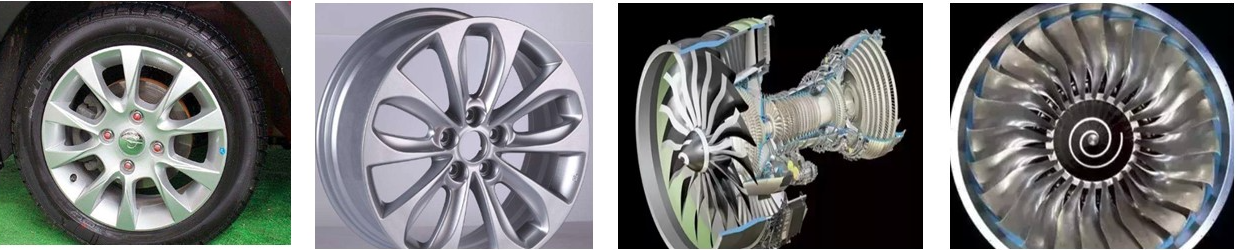
\includegraphics[width=0.95\textwidth]{Figure/有色金属材料.png}
\caption{有色金属材料示例}
\label{fig:有色金属材料}
\end{figure}

\subsubsection{非金属材料}

\begin{enumerate}
	\item \textbf{工程塑料}（尼龙、POM 聚甲醛等）：耐磨、自润滑，用于制造轻载齿轮、滑块；
	\item \textbf{橡胶}：用于减振、密封件；
	\item \textbf{陶瓷}：耐磨耐高温，用于特殊工况。
\end{enumerate}

\begin{figure}[H]
\centering
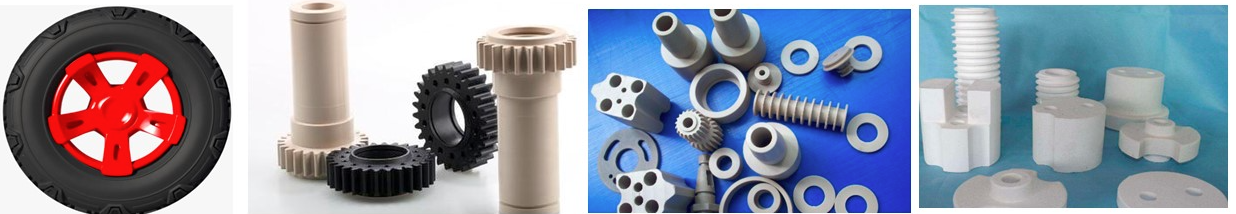
\includegraphics[width=0.95\textwidth]{Figure/非金属材料.png}
\caption{非金属材料示例}
\label{fig:非金属材料}
\end{figure}

\subsubsection{复合材料}

复合材料（如碳纤维复合材料、氧化陶瓷基复合材料等）由两种或多种性质不同的材料组合而成，具有纤维增强、轻质高强等特点，在航空航天等领域应用广泛。

\begin{figure}[H]
\centering
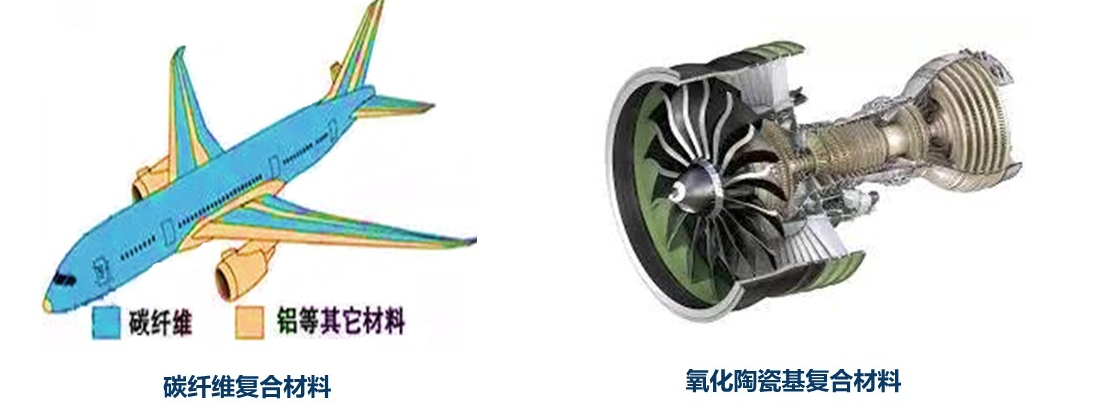
\includegraphics[width=0.9\textwidth]{Figure/复合材料.png}
\caption{复合材料在航空领域中的应用}
\label{fig:复合材料}
\end{figure}

\subsection{机械零件材料的选用要求}

\textbf{（1）使用要求。}根据零件的受载情况和工作状况、对零件尺寸和质量的限制、零件的重要程度等提出要求。

\textbf{（2）工艺要求。}要考虑毛坯制造、机械加工、热处理等工艺的可行性。

\textbf{（3）经济性要求。}考虑材料的相对价格、零件质量、加工性能及加工费用、材料的利用率，遵循局部品质原则，在性能相近时选用廉价的材料。

